\documentclass[a4paper,KOMA,landscape,titlepage]{powersem}
%\documentclass[letterpaper,KOMA,landscape,titlepage]{powersem}
\usepackage[stmo,button]{ifmslide}
\usepackage{graphicx}
%\usepackage{amsmath}
%\usepackage{amsfonts}
%\usepackage{listings}
%\usepackage[T1]{fontenc}
%\usepackage{mathptmx}
%\usepackage{charter}
%\usepackage{pictexwd}

%%%%%%%%%%%%%%%%%%%%%%%%%%%%%%%%%%%%%%%%%%%%%%%%%%%%%%%%%%%%%%%%%%%%
% Set some info on the pdf-file itself (optional)
%%%%%%%%%%%%%%%%%%%%%%%%%%%%%%%%%%%%%%%%%%%%%%%%%%%%%%%%%%%%%%%%%%%%
\hypersetup{pdfauthor={John Sibert}}
\hypersetup{pdfsubject={Assessment Model of MHI YFT Stocks}}
\hypersetup{pdftitle={Assessment model of Main Hawaiian Islands
Yellowfin Tuna Population}}
\hypersetup{pdfkeywords={yellowfin,state space, biomass transfer, model,Hawaii}}
\hypersetup{pdfpagemode=UseThumbs}
\hypersetup{bookmarks=false}
\newcommand\doublespacing{\baselineskip=1.6\normalbaselineskip}
\newcommand\singlespacing{\baselineskip=1.0\normalbaselineskip}
\renewcommand\deg[1]{$^\circ$#1}
\newcommand\SD{SEAPODYM}
\newcommand\MFCL{MULTIFAN-CL}
\newcommand\ADMB{ADModel Builder}
\newcommand\SPC{Secretariat of the Pacific Community}
\newcommand\WCPO{Western Central Pacific Ocean}
\newcommand\SSAP{Skipjack Survey and Assessment Programme}
\newcommand\RTTP{Regional Tuna Tagging Programme}
\newcommand\PTTP{Pacific Tuna Tagging Programme}
\newcommand\FAD{fish aggregating device}
\newcommand\ADRM{advection-diffusion-reaction model}
\newcommand\help[1]{\color{red}{\it #1 }\normalcolor}
\newcommand\widebar[1]{\overline{#1}}
\newcommand\EEZ{Exclusive Economic Zone}

\newcommand\None{{N_{1,1}}}
\newcommand\Ntwo{{N_{2,1}}}
\newcommand\Nsum{{N_{1,1}+N_{2,1}}}
\newcommand\peryr{yr$^{-1}$}
\newcommand\prevN[1]{{#1_{t-\Delta t}}}
\newcommand\nextN[1]{{#1_t}}

\begin{document}
\pageTransitionReplace
\pagecounter[on]
\slidepagestyle{empty}
\panelposition{outsidebottom}


%\freelogo(25,-13)[1.09cm] % outside bottom right of page counter
\freelogo(25,-13.8)[1.2cm] % outside bottom right of page counter

\definecolor{mytitle}{rgb}{0.0,0.4,0.5}
\definecolor{myauthor}{rgb}{0.9,0.9,0}
\definecolor{section1}{rgb}{0,0,.9}

%%%%%%%%%%%%%%%%%%%%%%%%%%%%%%%%%%%%%%%%%%%%%%%%%%%%%%%%%%%%%%%%%%%%
%\orgname{Universty of Hawaii}
%\orgname{Retirement-failure Consulting}
%\orgurl{http://admb-project.org/}

\author{\scalebox{1}[1.3]{John Sibert, Retirement-failure Consulting}} 
\title{Developing a stock assessment model for 
Main Hawaiian Islands Yellowfin Tuna Fishery}


\address{\href{mailto:sibert@hawaii.edu}{sibert@hawaii.edu}}

\begin{slide}
\maketitle
\end{slide}

%\begin{slide}
%\section{Feasibility of developing a stock assessment model for 
%Main Hawaiian Islands Yellowfin Tuna Fishery}
%\begin{center}
%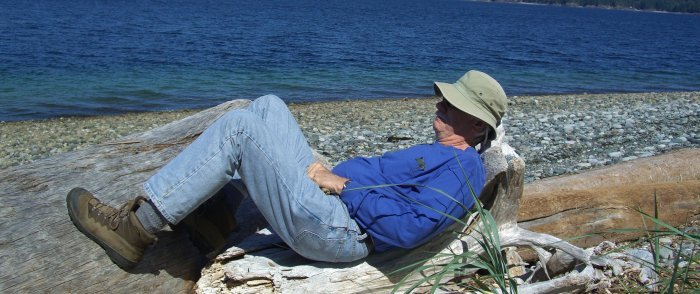
\includegraphics[width=0.7\textwidth]{./graphics/recumbant.png}
%~
%\vspace{2ex}
%{\color{author}
%\scalebox{1}[1.3]{John Sibert, Retirement-failure Consulting}
%\normalcolor}
%\end{center}
%\end{slide}

\centerslidesfalse
\begin{slide}\section{Model Assumptions}
\begin{enumerate}
\item The Pacific Ocean is divided into two regions:
MHI (1) and elsewhere (2).
\item Fish immigrate from region 2 to region 1, and mix completely.
\item Fish emigrate from region 1 to region 2, but have
no effect on region 2 dynamics.
\item Immigration into region 1 is dependent on biomass in region 2 estimated by
some other model, e.g., \MFCL\ or \SD.
\item The fishery comprises several gear types or fleets, each
characterized by a distinct fishing mortality time series.
\item Ninety percent of the fish resident in region 1 are assumed to
be locally spawned and reared.% (Wells et al 2012). 
%\item Population near ``equilibrium'' in 1952.
\end{enumerate}
\end{slide}

\begin{slide}\section{Combined HDAR and NOAA Catch Time Series}
\begin{center}
\begin{tabular}{cc}
Quarterly & First Differences of log(C)\\
\includegraphics[width=0.4\textwidth]{./graphics/5_gear_catch_history_q.pdf}&
\includegraphics[width=0.4\textwidth]{./graphics/first_difference_histograms.pdf}\\
\end{tabular}
\end{center}
\end{slide}

\begin{slide}\section{MFCL Biomass Estimates for MFCL Region 2}
\begin{center}
\includegraphics[width=0.8\textwidth]{./graphics/annual_region_2_biomass.pdf}
\end{center}
\end{slide}

\begin{slide}\section{Model Characteristics}
\begin{enumerate}
\item State-space model; separates process error from observation
error.
\begin{eqnarray}
\alpha_t &=&T(\alpha_{t-1}) + \eta_t\\
x_t &=& O(\alpha_t) + \varepsilon_t
\end{eqnarray}
\item Fishing mortality as random walk:~
$\log F_{g,t} = \log F_{g,t-1} + \xi_t;\quad \xi_t\sim
N(0,\sigma^2_\xi)$
\item Transition equation: Coupled logistic simultaneous ordinary
differential equation (\ref{eqn:coupledschaeferq})
\item Observation equation: robust likelihood (normal with 7\%
contamination by Cauchy) 
\item ``Off-line'' coupling to \MFCL\ region 2 biomass from 2014 assessment
\item Bayesian prior on proportion local:~$L(p)\sim
N(L(\bar{p}),\sigma^2_{L(p)})$
(\ref{fig:propLprior})
\item Model states are random effects
\end{enumerate}
\end{slide}

\begin{slide}\section{Model Parameters}
\begin{center}
\begin{tabular}{ll}
\hline
Variable & Definition\\
\hline
\hline
$r$ & Instantaneous growth rate $(y^{-1})$\\
$K$ & Asymptotic biomass (mt) \\
$T_{12}$ & Emigration rate $(y^{-1})$\\
$T^*_{21}$& Immigration rate $(y^{-1})$\\
$q$ & Nonlinear mortality apportionment proportion\\
\hline
$\sigma_\eta$ & Population growth standard deviation\\
$\sigma_\xi$ & Fishing mortality random walk standard deviation\\
$\sigma_\varepsilon$ & Observation error standard deviation \\
$a_g\; g=1\ldots n$ & Observation error contaminated by 
fat-tailed distribution\\
\hline
$\bar{p}$ & Mean proportion local\\
$\sigma_{L(p)}$ & Standard deviation logit transformed $\bar{p}$\\
\hline
\end{tabular}
\end{center}
\end{slide}

\begin{slide}\section{Stability Considerations --- Phase Plane Analysis}
\begin{center}
\includegraphics[width=\textwidth]{./graphics/qcomp_2.pdf}
\end{center}
\end{slide}

\begin{slide}\section{Simulated Populations}
\begin{center}
\begin{tabular}{ll}
~~~~~~~~~$q=0.48; \sigma_\eta=0$ &~~~~~~~~~$q=0.52; \sigma_\eta=0$\\
\includegraphics[width=0.5\textwidth]{./graphics/sim_q48_NNts.pdf}&
\includegraphics[width=0.5\textwidth]{./graphics/sim_q52_NNts.pdf}\\
\end{tabular}
\end{center}
\end{slide}

\begin{slide}\section{Simulated Populations with Process Error}
\begin{center}
\begin{tabular}{ll}
~~~~~~~~~$q=0.48; \sigma_\eta\sim 0.01$ &~~~~~~~~~$q=0.52;
\sigma_\eta\sim 0.01$\\
\includegraphics[width=0.5\textwidth]{./graphics/sim_q48r_NNts.pdf}&
\includegraphics[width=0.5\textwidth]{./graphics/sim_q52r_NNts.pdf}\\
\end{tabular}
\end{center}
\end{slide}

\begin{slide}\section{Estimation results: biomass}
\begin{center}
\includegraphics[height=0.85\textheight]{./graphics/est_popB25.pdf}
\end{center}
\end{slide}

\begin{slide}\section{Estimation results: fishery}
\begin{center}
\begin{tabular}{cc}
{\tiny Fishing Mortality} & {\tiny Catch}\\
\includegraphics[width=0.40\textwidth]{./graphics/est_FB25.pdf}&
\includegraphics[width=0.40\textwidth]{./graphics/est_catchB25.pdf}\\
\end{tabular}
\end{center}
\end{slide}

\begin{slide}\section{Estimation results: parameter values}
{\renewcommand{\arraystretch}{0.8}
\begin{center}
\begin{tabular}{lrr}
\hline
Variable & Initial Value & Final Value\\
\hline
$r$ & 1.20&  1.30\\
$K$ & 150,000 & 151,000 \\
$T_{12}$ & 0.01 & 0.00999\\
$T^*_{21}$& 0.002 & 0.00199\\
$q$ & 0.54 & 0.525\\
\hline
$\sigma_\eta$ & 0.1 & 0.0880\\
$\sigma_\xi$ & 0.3 & 0.700\\
$\sigma_\varepsilon$ & 1.0 & 0.0913\\
$a_1$ & 0.07 & ---\\
$a_2$ & 0.07 & ---\\
$a_3$ & 0.07 & ---\\
$a_4$ & 0.07 & ---\\
$a_5$ & 0.07 & ---\\
\hline
$\bar{p}$ & 0.9 & ---\\
$\sigma_{\bar{p}}$ & 0.8 & ---\\
\hline
\end{tabular}
\end{center}
}
\end{slide}

\begin{slide}\section{Simulation: 100 X Fishing Mortality}
\begin{center}
\begin{tabular}{cc}
\includegraphics[width=0.45\textwidth]{./graphics/sim_F100_NNts.pdf}&
\includegraphics[width=0.45\textwidth]{./graphics/est_sim_F100_popB19.pdf}
\end{tabular}
\end{center}
\end{slide}

\begin{slide}\section{Estimation: 100 X Fishing Mortality}
{\renewcommand{\arraystretch}{0.8}
\begin{center}
\begin{tabular}{lrr}
\hline
Variable & Initial Value & Final Value\\
\hline
$r$ & 1.20&  0.190\\
$K$ & 200,000 & 1,030,000 \\
$T_{12}$ & 0.01 & 0.00524\\
$T^*_{21}$& 0.02 & 0.00128\\
$q$ & 0.54 & 0.511\\
\hline
$\sigma_\eta$ & 0.1 & 0.00231\\
$\sigma_\xi$ & 0.3 & 0.704\\
$\sigma_\varepsilon$ & 1.0 & 0.367\\
$a_1$ & 0.07 & ---\\
$a_2$ & 0.07 & ---\\
$a_3$ & 0.07 & ---\\
$a_4$ & 0.07 & ---\\
$a_5$ & 0.07 & ---\\
\hline
$\bar{p}$ & 0.9 & ---\\
$\sigma_{\bar{p}}$ & 0.8 & ---\\
\hline
\end{tabular}
\end{center}
}
\end{slide}

\begin{slide}\section{Conclusions}
What works:
\begin{itemize}
\item Random walk representation of fishing mortality
\item Bayesian constraint on $\bar{p}$
\item Off-line coupling 
\item Robust likelihood
\item State-space framework
\end{itemize}
Not working:
\begin{itemize}
\item Estimation procedure does not terminate normally
\item Numerical instability in numerical approximation
\end{itemize}
\end{slide}

\begin{slide}\section{Issues:}
\begin{itemize}
\item Convergence, or lack thereof.
\item Is $\bar{p} = 0.9$ since 1952?
\item If so, are two subpopulations necessary?
\item Intra annual variability caused by abundance, participation,
reporting, weather, ... ?
\item Recreational data? How to represent errors in observation
equation?
\item Should an age-structured model be developed?
\item What are appropriate reference points for a stock segment?
\item Use MFCL estimates as abundance index?
\end{itemize}
\end{slide}

\begin{slide}\section{Back to the drawing board ...}
\begin{center}
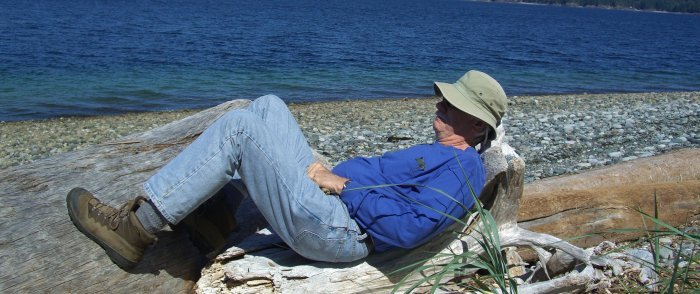
\includegraphics[width=0.8\textwidth]{./graphics/recumbant.png}
\end{center}
\end{slide}

%%%%%%%%%%%%%%%%%%%%%%%%%%%%%%%%%%%%%%%%%%%%%%%%%%%%%%%%%%%%%%%%%%%%

\begin{slide}\section{Logistic Dynamics}
\begin{center}
\begin{equation}
\frac{d}{dt}\big(\Nsum\big)=\big(\Nsum\big)\Big[r\Big(1-\frac{\Nsum}{K}\Big)-F-T_{12}\Big]+T_{21}
\label{eqn:logistic}
\end{equation}
\vspace{2ex}

\begin{eqnarray}
\label{eqn:coupledschaeferq}
\frac{d\None}{dt}&=&\None\Big[r\Big(1-\frac{\None}{K}\Big)
-F - T_{12}\Big] - (1-q)2r\frac{\None\Ntwo}{K}\nonumber\\
\\
\frac{d\Ntwo}{dt}&=&\Ntwo\Big[r\Big(1-\frac{\Ntwo}{K}\Big)
-F - T_{12}\Big] - q2r\frac{\None\Ntwo}{K} + T_{21}\nonumber
\end{eqnarray}
\end{center}
\end{slide}

\begin{slide}\section{State-space Transition Equation}
\begin{center}
\begin{equation}
\alpha_t=T(\alpha_{t-1}) + \eta_t
\end{equation}
\vspace{2ex}
\begin{eqnarray}
\label{eqn:finitecoupledlogschaefer}
\log \None_t &=& \log \None_{t-\Delta t}\nonumber\\ 
             &+&\Delta t\bigg(r\Big(1-\frac{\None_{t-\Delta t}}{K}\Big)
-\sum_{g=1}^n F_{g,t-\Delta t} - T_{12} - (1-q)2r\frac{\Ntwo_{t-\Delta
t}}{K}\bigg)+\eta_t\nonumber\\
\\ \log \Ntwo_t &=& \log \Ntwo_{t-\Delta t}\nonumber\\
             &+&\Delta t\bigg(r\Big(1-\frac{\Ntwo_{t-\Delta t}}{K}\Big)
-\sum_{g=1}^n F_{g,t-\Delta t} - T_{12} - q2r\frac{\None_{t-\Delta t}}{K}
     +\frac{T_{{21}_{t-\Delta t}}}{\Ntwo_{t-\Delta t}}\bigg)+\eta_t\nonumber
\end{eqnarray}
\end{center}
\end{slide}

\begin{slide}\section{State-space Observation Equation}
\begin{center}
\begin{equation}
x_t = O(\alpha_t) + \varepsilon_t
\end{equation}
\vspace{2ex}
\begin{equation}
\log C_{g,t} = \log \Biggl(F_{g,t}\cdot\Bigl(\frac{\None_{t-\Delta t}+\None_t}{2}
                           +\frac{\Ntwo_{t-\Delta
t}+\Ntwo_t}{2}\Bigr)\Biggr) + \varepsilon_t
\label{eqn:obs}
\end{equation}
\begin{equation}
\varepsilon_t \sim
(1-a_g)*N(0,\sigma^2_\varepsilon)+a_g*C(0,\sigma^2_\varepsilon);\quad a_g =
0.07
\end{equation}
\end{center}
\end{slide}

\begin{slide}\section{Proportion Local Prior}
\begin{center}
\label{fig:propLprior}
\includegraphics[height=0.80\textheight]{./graphics/propL_prior.pdf}
\end{center}
\end{slide}
\end{document}

